%=====================================================================
%  GROUP 1 -- Designing and Deploying Data Pipelines
%  Student-led lesson skeleton. Data Wrangling, Fall 2026.
%  Compile:  latexmk -pdf Group1_Lesson_Skeleton.tex
%=====================================================================
\documentclass[11pt]{article}

\usepackage[margin=0.9in,top=0.85in,bottom=0.9in]{geometry}
\usepackage[T1]{fontenc}
\usepackage[utf8]{inputenc}
\usepackage{xcolor}
\usepackage[most]{tcolorbox}
\usepackage{enumitem}
\usepackage{titlesec}
\usepackage{booktabs}
\usepackage{tikz}
\usetikzlibrary{positioning,arrows.meta}
\usepackage{fancyhdr}
\usepackage[hidelinks]{hyperref}

\definecolor{ink}{HTML}{1B2631}
\definecolor{brand}{HTML}{1F4E79}
\definecolor{accent}{HTML}{C0392B}
\definecolor{good}{HTML}{1E8449}
\definecolor{soft}{HTML}{F4F6F7}
\definecolor{grayish}{HTML}{5D6D7E}

\titleformat{\section}{\Large\bfseries\color{brand}}{\thesection}{0.6em}{}
\titleformat{\subsection}{\large\bfseries\color{ink}}{\thesubsection}{0.6em}{}
\titlespacing*{\section}{0pt}{16pt}{8pt}
\titlespacing*{\subsection}{0pt}{12pt}{5pt}

\pagestyle{fancy}\fancyhf{}
\lhead{\small\color{grayish}Data Wrangling F26 · Group 1}
\rhead{\small\color{grayish}Data Pipelines \& Orchestration}
\cfoot{\small\color{grayish}\thepage}
\renewcommand{\headrulewidth}{0.4pt}

\setlist[itemize]{leftmargin=1.4em,topsep=3pt,itemsep=2pt}
\setlist[enumerate]{leftmargin=1.6em,topsep=3pt,itemsep=2pt}

% ---------------- boxes ----------------
\newtcolorbox{qbox}[1][]{
  enhanced, breakable, colback=brand!4, colframe=brand,
  boxrule=0pt, leftrule=3pt, arc=1pt,
  title={\bfseries\color{brand}Questions you must answer in your slides},
  fonttitle=\normalsize, coltitle=brand, colbacktitle=brand!4,
  attach boxed title to top left={xshift=6pt,yshift=-2pt},
  boxed title style={colframe=brand!4,boxrule=0pt},
  top=16pt, #1}

\newtcolorbox{dobox}[1][]{
  enhanced, breakable, colback=good!5, colframe=good,
  boxrule=0pt, leftrule=3pt, arc=1pt, #1}

\newtcolorbox{warnbox}[1][]{
  enhanced, breakable, colback=accent!5, colframe=accent,
  boxrule=0pt, leftrule=3pt, arc=1pt, #1}

\newtcolorbox{codebox}[1][]{
  enhanced, breakable, colback=soft, colframe=grayish!40,
  boxrule=0.4pt, arc=1pt, fontupper=\ttfamily\small, #1}

\newcommand{\key}[1]{\textcolor{accent}{\textbf{#1}}}
\newcommand{\tm}[1]{\textcolor{grayish}{\small\textsf{[#1]}}}

\begin{document}

%=====================================================================
\begin{center}
{\color{grayish}\small DATA WRANGLING · FALL 2026 · STUDENT-LED LESSON}\\[6pt]
{\Huge\bfseries\color{brand} Group 1}\\[6pt]
{\LARGE\bfseries\color{ink} Designing and Deploying Data Pipelines}\\[4pt]
{\large\color{ink} Introduction to Orchestration Frameworks (Airflow, Luigi)}\\[10pt]
\rule{\textwidth}{1pt}
\end{center}

\vspace{-4pt}
\begin{center}
\begin{tabular}{@{}ll@{}}
\textbf{Class time you own:} & 50 minutes \\
\textbf{You hand in:} & slides + a working live demo \\
\textbf{You build:} & a scheduled, idempotent pipeline over the \textit{Bison Bikes} data \\
\textbf{Environment:} & your own laptop, \texttt{pip} only (no Docker) \\
\end{tabular}
\end{center}
\vspace{6pt}

\begin{dobox}
\textbf{Read this first.} This is a \emph{skeleton}, not a lesson. Every
section below tells you what the class needs to learn and asks you questions.
\key{Your job is to answer the questions and turn the answers into the lesson.}
Nothing here is written out for you to read aloud --- if you find yourself
reading this document to the class, you have misunderstood the assignment.

You are the instructors for 50 minutes. Teach it.
\end{dobox}

%=====================================================================
\section{What you are handing in}

\begin{enumerate}
  \item \textbf{Slides} covering Sections 3--4 of this document. Roughly
        12--18 slides. Every concept slide must have a concrete example on it,
        not just a definition.
  \item \textbf{A live demo} of a pipeline \emph{you} built, running on your
        laptop, in front of the class. It must actually run. A video recording
        is an acceptable backup, but you lose points if you never attempt it live.
  \item \textbf{Your code}, emailed to the instructor before class starts.
\end{enumerate}

\begin{warnbox}
\textbf{The single most common failure of this assignment} is a group that
spends all its time fighting the installation and arrives with a great
explanation and nothing to show. \key{Do Section 2 in the first 48 hours.}
If Airflow will not install on your machine by the end of week one, switch to
the Luigi path and spend your remaining time on the teaching.
\end{warnbox}

%=====================================================================
\section{Setup --- do this first, not the night before}

\subsection*{Path A (preferred): Airflow}

\begin{codebox}
python3 -m venv .venv \&\& source .venv/bin/activate\\
pip install "apache-airflow==3.1.3" pandas\\
export AIRFLOW\_HOME=\$(pwd)/airflow\_home\\
airflow standalone
\end{codebox}

\noindent
\texttt{airflow standalone} starts the scheduler, the API server and a web UI
in one process and prints an admin password. Open
\texttt{http://localhost:8080}. Put \texttt{bikeshare\_dag.py} and
\texttt{transforms.py} in \texttt{\$AIRFLOW\_HOME/dags/}.

\begin{warnbox}
\textbf{Windows:} Airflow does not support native Windows. Use WSL2 (Ubuntu),
or take Path B. Do not lose three days to this.\\[3pt]
\textbf{macOS:} if you hit a \texttt{fork()} crash during task execution, run
\texttt{export OBJC\_DISABLE\_INITIALIZE\_FORK\_SAFETY=YES} before
\texttt{airflow standalone}.
\end{warnbox}

\subsection*{Path B (fallback): Luigi}

\begin{codebox}
pip install luigi pandas\\
python bikeshare\_luigi.py --local-scheduler LoadWarehouse --ds 2026-09-01
\end{codebox}

\noindent
One install, no database, no server, works everywhere. You lose the UI, the
scheduler and backfill --- and \key{explaining exactly what you lost is worth
more to the class than having used the fancier tool}. If you take this path,
Section 4.5 becomes the centrepiece of your lesson instead of a footnote.

\subsection*{Verify your data}

\begin{codebox}
ls data/raw/\\
\# rides\_2026-09-01.csv ... rides\_2026-09-07.csv, weather\_2026-09.csv, stations.csv
\end{codebox}

%=====================================================================
\section{The lesson you must teach}

Five concept blocks. Together they are about 25 minutes of your 50. For each
one: the \textbf{required content} is the floor, and the \textbf{questions} are
what you must actually answer on a slide.

%---------------------------------------------------------------
\subsection{What a data pipeline is \tm{3 min}}

\textbf{Required content.} Define a pipeline as a sequence of dependent
transformations moving data from a source to a destination. Define
\key{ETL} and \key{ELT} and draw both. Name where our Bison Bikes build sits.

\begin{qbox}
\begin{enumerate}
  \item ETL transforms before loading; ELT loads raw data first and transforms
        inside the warehouse. Give one concrete reason a team would choose each.
  \item Which one is our Bison Bikes pipeline, and why does the fact that we
        stage the raw file \emph{untouched} before cleaning it matter?
  \item A classmate says ``why not just clean the data as we read it and skip
        the staging step?'' Answer them.
\end{enumerate}
\end{qbox}

%---------------------------------------------------------------
\subsection{Why orchestration exists: the cron problem \tm{5 min}}

This is the \textbf{motivating failure} of your whole lesson. Do not skip it
and do not rush it. Everything after this is a response to this slide.

\textbf{Required content.} Present this script and tear it apart:

\begin{codebox}
\# crontab: run every day at 2am\\
0 2 * * * python /home/me/run\_pipeline.py >> /tmp/log.txt 2>\&1
\end{codebox}

\begin{qbox}
Name what breaks, specifically. At minimum, answer all six:
\begin{enumerate}
  \item The source file for Tuesday lands at 2:07am instead of 1:50am. What
        happens, and how would you find out?
  \item The job fails on Tuesday. Wednesday runs fine. Tuesday's data is now
        missing forever. How does cron help you notice? (It does not. Say why.)
  \item You fix a bug and need to re-process all of September. What do you type?
  \item Step 4 of 7 fails. The first three already wrote to the database.
        What state is your warehouse in now?
  \item Two runs overlap because yesterday's took three hours. What happens?
  \item Someone asks ``did last Thursday's load succeed?'' Where do you look?
\end{enumerate}
\end{qbox}

\begin{dobox}
\textbf{Teaching move that works:} ask the class to solve problem 3 with cron
before you reveal that \texttt{airflow dags backfill} is one command. Let them
feel the problem for 60 seconds first.
\end{dobox}

%---------------------------------------------------------------
\subsection{DAGs \tm{4 min}}

\textbf{Required content.} Directed, acyclic, graph --- define each word and
say why each is load-bearing. Draw the Bison Bikes DAG on a slide:

\begin{center}
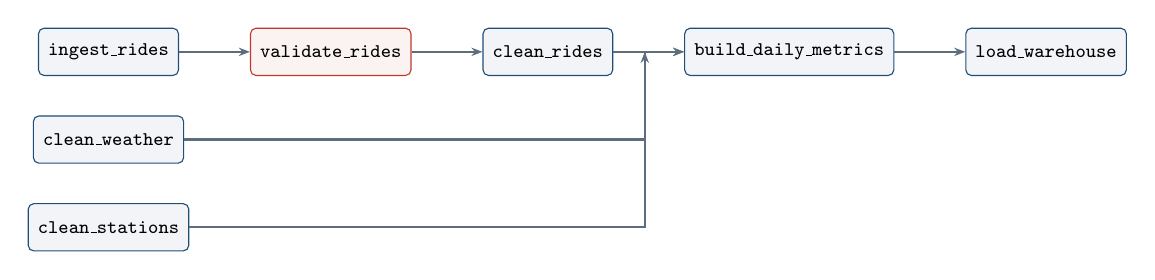
\begin{tikzpicture}[
   node distance=5mm and 9mm,
   t/.style={rectangle,rounded corners=2pt,draw=brand,fill=brand!6,
             font=\scriptsize\ttfamily,inner sep=3.5pt,minimum height=6mm},
   g/.style={t,draw=accent,fill=accent!6},
   a/.style={-{Stealth[length=4pt]},draw=grayish,thick}]
  \node[t] (i)  {ingest\_rides};
  \node[g,right=of i] (v) {validate\_rides};
  \node[t,right=of v] (c) {clean\_rides};
  \node[t,below=of i] (w) {clean\_weather};
  \node[t,below=of w] (s) {clean\_stations};
  \node[t,right=of c] (b) {build\_daily\_metrics};
  \node[t,right=of b] (l) {load\_warehouse};
  \draw[a] (i)--(v); \draw[a] (v)--(c); \draw[a] (c)--(b);
  \draw[a] (w) -| ([xshift=-5mm]b.west) -- (b.west);
  \draw[a] (s) -| ([xshift=-5mm]b.west);
  \draw[a] (b)--(l);
\end{tikzpicture}
\end{center}

\begin{qbox}
\begin{enumerate}
  \item Why must it be \emph{acyclic}? Describe what an orchestrator would do
        if you gave it a cycle.
  \item \texttt{clean\_weather} and \texttt{clean\_stations} can start
        immediately. \texttt{clean\_rides} cannot. Why?
  \item If you had 8 workers available, how many of these 7 tasks could run at
        the same instant? Which ones?
  \item The red task is a \key{quality gate}. What should the DAG do if it
        fails --- and what should it specifically \emph{not} do?
\end{enumerate}
\end{qbox}

%---------------------------------------------------------------
\subsection{The four properties that make a pipeline production-grade \tm{8 min}}

This is the technical core of the lesson. Give each one its own slide, each
with a concrete example from your own build.

\begin{center}
\small
\begin{tabular}{@{}p{0.2\textwidth}p{0.74\textwidth}@{}}
\toprule
\textbf{Property} & \textbf{What it means, and where it shows up in your build} \\
\midrule
\key{Idempotency} &
Running the same task twice produces the same result as running it once. Our
\texttt{load\_warehouse} deletes the row for that date before inserting. You
will demo this live. \\
\addlinespace
\key{Retries} &
Transient failures (a file has not landed, the network blipped) should be
retried automatically. Permanent failures (bad schema) should not. Your DAG
sets \texttt{retries} and \texttt{retry\_delay}. \\
\addlinespace
\key{Backfill} &
One DAG definition must be able to process any date, including past ones. This
is why every task takes \texttt{ds} and nothing hard-codes a filename. \\
\addlinespace
\key{Observability} &
Someone who is not you must be able to answer ``did it run, did it work, how
long did it take, and what broke'' without reading your code. \\
\bottomrule
\end{tabular}
\end{center}

\begin{qbox}
\begin{enumerate}
  \item Idempotency is the hard one. Classify each of these as idempotent or
        not, and fix the ones that are not:
        \begin{itemize}
          \item \texttt{INSERT INTO daily\_metrics VALUES (...)}
          \item \texttt{df.to\_csv("out.csv")}
          \item \texttt{df.to\_csv("out.csv", mode="a")}
          \item \texttt{UPDATE accounts SET balance = balance - 50}
        \end{itemize}
  \item Why is the last one the scariest of the four?
  \item Our \texttt{ingest\_rides} raises \texttt{FileNotFoundError} when the
        source has not delivered. Should that be retried? For how long? What
        should happen when the retries run out?
  \item \texttt{catchup=True} with a \texttt{start\_date} of 2019 would launch
        thousands of runs the moment you unpause the DAG. Explain to the class
        why this is one of the most common ways people take down their own
        Airflow instance.
\end{enumerate}
\end{qbox}

%---------------------------------------------------------------
\subsection{The framework landscape \tm{5 min}}

\textbf{Required content.} The class should leave able to say what each tool is
\emph{for}, not just that it exists. Build this table and defend your entries.

\begin{center}
\small
\begin{tabular}{@{}llp{0.42\textwidth}@{}}
\toprule
\textbf{Tool} & \textbf{Model} & \textbf{Use it when\ldots} \\
\midrule
Airflow  & task-based, scheduler-driven & \emph{you fill this in} \\
Luigi    & target-based (a task is done if its output exists) & \emph{you fill this in} \\
Prefect  & Python-native, dynamic DAGs & \emph{you fill this in} \\
Dagster  & asset-based (you declare the data, not the task) & \emph{you fill this in} \\
dbt      & SQL transformations inside the warehouse & \emph{you fill this in} \\
\bottomrule
\end{tabular}
\end{center}

\begin{qbox}
\begin{enumerate}
  \item Airflow asks ``what tasks must run and when?'' Luigi asks ``what output
        do I want, and what is missing?'' Explain how Luigi's model gives you
        idempotency almost for free --- and what it costs you.
  \item Dagster calls itself asset-based rather than task-based. What is the
        difference, in one sentence a classmate would understand?
  \item dbt does not move data at all. So why is it in every modern data stack
        diagram?
  \item \textbf{Required opinion slide.} Your team has three people, one
        warehouse, and twelve daily jobs. Pick one tool. Defend it in 30
        seconds. There is no wrong answer, only an undefended one.
\end{enumerate}
\end{qbox}

%=====================================================================
\section{The build}

You are implementing a pipeline over \textit{Bison Bikes}, a campus bike-share
system. Seven days of ride files, one weather file, one station file.

\subsection{What is wrong with the data (on purpose)}

\begin{center}
\small
\begin{tabular}{@{}llp{0.42\textwidth}@{}}
\toprule
\textbf{File} & \textbf{Defect} & \textbf{What your pipeline must do} \\
\midrule
\texttt{rides\_*.csv} & \texttt{duration\_min = 9999} & sentinel, not a measurement \\
 & negative durations & impossible \\
 & \texttt{member\_age = 999} & sentinel \\
 & \texttt{end\_time < start\_time} & impossible ordering \\
 & duplicate \texttt{ride\_id} & re-delivered rows; tests your dedupe \\
 & station \texttt{ST99} & referential integrity --- no such station \\
\addlinespace
\texttt{weather\_2026-09.csv} & two rows in Fahrenheit & convert, do not delete \\
 & \texttt{precip\_mm = -999} & sentinel \\
 & \textbf{2026-09-05 missing} & decide what the join does. Do not invent it. \\
\addlinespace
\texttt{stations.csv} & \texttt{ST03} appears twice & deduplicate \\
 & whitespace/case variants & normalise \\
 & \texttt{capacity = 0}, missing coords & decide and document \\
\bottomrule
\end{tabular}
\end{center}

\begin{dobox}
This is the same class of problem as the outlier and data-quality lesson.
\key{Your quality gate is where that lesson becomes infrastructure.} Make that
connection explicitly in your slides --- it is worth points.
\end{dobox}

\subsection{Your TODO list}

\begin{enumerate}
  \item Fill in the six functions in \texttt{transforms.py}.
  \item Fill in the DAG settings and task wiring in \texttt{bikeshare\_dag.py}.
  \item Run it for one day. Then backfill all seven.
  \item Re-run one day twice and prove the warehouse did not duplicate.
  \item Lower \texttt{QUALITY\_THRESHOLD} to \texttt{0.02} and watch the gate
        fail. \key{Keep that screenshot.} The failing run is a better slide
        than the passing one.
\end{enumerate}

\begin{qbox}
\begin{enumerate}
  \item Your quality gate fires at 2\%. What is the right threshold, and how
        would you decide it rather than guessing?
  \item 2026-09-04 has roughly half the rides of other weekdays. Before you
        look: is that a data problem or a real effect? Check the weather file
        and tell the class what you found.
  \item \texttt{transforms.py} imports neither Airflow nor Luigi. Why was that
        a deliberate design choice, and what does it buy you? (Hint: how would
        you unit-test \texttt{clean\_rides}?)
  \item You ran the same pipeline through two different frameworks. What was
        identical and what changed?
\end{enumerate}
\end{qbox}

%=====================================================================
\section{Your 50 minutes}

A plan that fits. Adjust it, but hand in \emph{a} plan.

\begin{center}
\small
\begin{tabular}{@{}rp{0.52\textwidth}p{0.26\textwidth}@{}}
\toprule
\textbf{Min} & \textbf{What happens} & \textbf{Who} \\
\midrule
0--3   & Hook: the 2am cron script. Ask what breaks. Take answers. & \\
3--6   & Pipelines, ETL vs ELT & \\
6--11  & The cron problem, all six failures & \\
11--15 & DAGs, draw yours & \\
15--23 & The four properties, one slide each & \\
23--28 & Framework landscape + your opinion slide & \\
\midrule
28--42 & \textbf{LIVE DEMO} (next page) & \\
\midrule
42--48 & Class activity: hand out the four idempotency snippets, 3 min in pairs, then discuss & \\
48--50 & Close: the one thing you want them to remember & \\
\bottomrule
\end{tabular}
\end{center}

\subsection{Live demo script \tm{14 min}}

Rehearse this end to end at least twice. Have the terminal font large enough
to read from the back row.

\begin{enumerate}
  \item \textbf{Start Airflow, open the UI.} Show the DAG list. \tm{1 min}
  \item \textbf{Show the graph view.} Point at the three parallel roots
        converging. Connect it to the slide you drew. \tm{2 min}
  \item \textbf{Trigger one day.} Watch the tasks go green in order. \tm{2 min}
  \item \textbf{Open a task's log} from the UI. This is observability --- make
        the point out loud. \tm{1 min}
  \item \textbf{Break it on purpose.} Lower the quality threshold to 2\% and
        re-run. The gate goes red, downstream tasks go yellow (upstream
        failed) and \emph{never run}. \key{This is the best 90 seconds of your
        demo.} \tm{2 min}
  \item \textbf{Fix it and clear the failed task} from the UI to re-run just
        that branch. \tm{1 min}
  \item \textbf{Backfill all seven days.} Show the grid filling in. \tm{3 min}
  \item \textbf{Prove idempotency.} Query the warehouse row count, re-run one
        day, query again. Same number. Say why. \tm{2 min}
\end{enumerate}

\begin{warnbox}
\textbf{Demo insurance.} Before class: take screenshots of every step above and
put them at the end of your deck. If the live demo dies, you switch to
screenshots and keep talking. Groups that do this never lose points for a
failed demo. Groups that do not, do.
\end{warnbox}

%=====================================================================
\section{Questions your classmates will ask}

Prepare answers. Two of these will come up.

\begin{enumerate}
  \item ``Isn't this just a Makefile?'' (It is closer than you think. What does
        Airflow add?)
  \item ``What if a task needs to run on a different machine?''
  \item ``How do you pass actual data between tasks?'' (Look up XCom --- and
        find out why passing a large DataFrame through it is a bad idea.)
  \item ``What happens if the scheduler itself dies mid-run?''
  \item ``Why is the start date in the past?''
  \item ``Can two DAGs depend on each other?''
\end{enumerate}

%=====================================================================
\section{How you will be graded}

\begin{center}
\small
\begin{tabular}{@{}p{0.30\textwidth}rp{0.44\textwidth}@{}}
\toprule
\textbf{Component} & \textbf{Pts} & \textbf{What full marks looks like} \\
\midrule
Conceptual teaching & 30 &
The cron problem lands. The class can define idempotency afterwards. \\
Live demo & 25 &
It runs. The failure case is shown deliberately, not accidentally. \\
Code quality & 15 &
Transforms are framework-free and readable. Idempotency is real, not claimed. \\
Questions answered & 15 &
The boxed questions are addressed on slides, not hand-waved. \\
Class engagement & 10 &
You asked the room something and waited for an answer. \\
Timing & 5 &
You finished within 50 minutes without cutting the demo. \\
\midrule
\textbf{Total} & \textbf{100} & \\
\bottomrule
\end{tabular}
\end{center}

\vspace{6pt}
\begin{dobox}
\textbf{The bar for an A:} by the end of your 50 minutes, a classmate who has
never heard of Airflow can explain to someone else \emph{why} a scheduled
script is not a pipeline. If they can only recite that Airflow uses DAGs, you
taught the vocabulary and skipped the lesson.
\end{dobox}

\end{document}
